\documentclass[11pt,a4paper]{article}
\usepackage{fontspec}
\usepackage{verbatim}
\usepackage{polyglossia}
\usepackage{titlesec}
\usepackage[left=2cm,top=1cm,right=2cm,bottom=16mm]{geometry}
\usepackage{fancyhdr}
\usepackage{xcolor}
\usepackage{indentfirst}
\usepackage{graphicx}
\usepackage{tabu}
\usepackage{longtable}
\usepackage{pbox}
\usepackage{pdfpages}
\setmainfont[Ligatures=TeX,ItalicFont={EBGaramond08-Italic.ttf},SmallCapsFont={EBGaramondSC08-Regular.ttf},BoldFont={LinLibertine_RB.otf}]{EBGaramond08-Regular.ttf}
\setmonofont{Courier New}
\setmainlanguage{czech}

\definecolor{high}{rgb}{0,0,1}
\definecolor{low}{rgb}{.03,.02,.72}
\definecolor{lower}{rgb}{.09,0,.52}
\definecolor{lowest}{rgb}{.45,.04,.52}
\definecolor{spell}{rgb}{.08,0,.67}

\def\clqq{„}
\def\crqq{“}
\def\clq{‚}
\def\crq{‘}
\def\Si{ſ}

\newcommand{\spell}[1]{{\small\scshape\color{spell} #1}}
\newcommand{\emp}[1]{{\fontspec[Ligatures=TeX]{Linux Libertine O} \emph{#1}}}

\setcounter{secnumdepth}{0}

\begin{document}
\pagestyle{fancy}
\fancyhf{}
\renewcommand{\headrulewidth}{0pt}
\fancyfoot[C]{\thepage}

\titleformat*{\section}{\huge\centering\fontspec[Ligatures=TeX]{Xirwena}\color{high}}
\titleformat*{\subsection}{\huge\scshape\color{low}}
\titleformat*{\subsubsection}{\Large\scshape\color{lower}}
\titleformat*{\paragraph}{\scshape\color{lowest}}

\newenvironment{cdescription}{
\begin{description}
\setlength{\itemsep}{0.1cm}
\setlength{\parskip}{0cm}
\setlength{\parsep}{0cm}}{\end{description}}
\newenvironment{cenumerate}{
\begin{enumerate}
\setlength{\itemsep}{0.1cm}
\setlength{\parskip}{0cm}
\setlength{\parsep}{0cm}}{\end{enumerate}}
\newenvironment{citemize}{
\begin{itemize}
\setlength{\itemsep}{0.1cm}
\setlength{\parskip}{0cm}
\setlength{\parsep}{0cm}}{\end{itemize}}
\newcommand{\cara}{\rule{\linewidth}{0.4mm}}

\begin{comment}
\begin{titlepage}
\begin{center}

{\Large \textsc{Federico Moreno Torroba}} \\[1.2cm]

\cara \\[0.5cm]
{\huge \textbf{Španělské hrady}} \\[0.6cm]
{\Large („Castillos de España“)} \\[6mm]
\cara \\[1.2cm]

\end{center}

{\large \textbf{Sazba}: \textsc{D. Cidlinský}}\\[1cm]

\begin{center}
{\huge\scshape Seznam skladeb}\\[6mm]
\end{center}

Alcañiz (2)

Alcázar de Segovia (3)

Calatrava (4,5)

Javier (6)

Olite (7,8)

Redaba (9)

Turégano (10, 11)

Alba de Tormes, Manzanares del Real (12)

Sigüenza, Torrija (13)

Montemayor (Romance de los Pinos), Simancas (14)

Zafra (15, 16)
\vfill
\end{titlepage}

\subsection{Poznámky k notaci}

Způsob, kterým jsem noty provedl, se může někomu zdát mírně netradiční. Mám tedy za to, že je vhodné říci k tomu pár slov.

První věc, které si čtenář všimne, je, že nerad otáčím při hraní papíry. Většina skladeb je proto směstnána na jedinou stránku (někdy se vejde skladba i na půl stránky), jen ty nejdelší mají výjimku. Někdy se zdá, že je výsledkem příliš zhuštěná notace (třeba u skladby \emph{Alcázar de Segovia}), ale pro mě je lepší mít trochu hustší notaci na jednom papíře než velmi řídkou na dvou. Většina skladeb se ale vejde do svého vymezeného místa velmi pohodlně.

Druhou záležitostí je rozsáhlé používání různých opakovacích struktur (repetice s několika „voltami“ (prima, secunda, tertia volta), popřípadě D. C. al Coda). Nenechte se překvapit větším množstvím volt (někdy až 4). Z méně tradiční notace je nutno zmínit procentové opakování (pokud v taktu vidíte jen symbol připomínající procento, znamená to, že se tam má hrát totéž co v taktu předchozím) a notaci „tremolo“ (pokud najdete čtvrťovou či delší notu přeťatou jedním či více trámci, znamená to, že máte hrát noty podle počtu trámců (je-li jeden, osminky, jsou-li dva, šestnáctinky atd.) tak dlouho, dokud jimi nenaplníte hodnotu uvedené noty. Celou dobu přitom hrajete týž tón. Třeba ve skladbě \emph{Turégano} je něco takového hned na počátku --- půlová nota s jedním trámcem znamená vlastně čtyři osminky (osminky se mají hrát tak dlouho, dokud nenaplní půlku)). Aby nedošlo kvůli tomu k nějakému nedorozumění, je v prvním taktu tremolo vždy plně rozepsáno (takže pak můžete hrát „podle vzoru“) a použití zkrácené notace je, jak bývá zvykem, označeno poznámkou „\emph{Simile}“.

Posuvky platí jen ve své vlastní oktávě, a to nejpozději jen do konce taktu, v němž byly uvedeny, popřípadě i kratší dobu, pokud je nahradí v průběhu daného taktu posuvka jiná. Změna dvojité posuvky na jednoduchou se děje bez uvedení odrážky a její odražení se provádí jen jedinou odrážkou, nikoli dvěma. Odrážky nikdy neodrážejí posuvky z předchozích taktů, jak se často vidí v klavírní hudbě. Předznamenání samozřejmě platí stále a ve všech oktávách.

Ve výběru posuvek jsem maximálně využíval enharmonických záměn a snažil se vždy zaznamenat tóny tak, aby bylo posuvek co nejméně. Někdy kvůli tomu dojde i k momentální změně předznamenání. Dvojité posuvky potírám (milost se jim dává, jen kdyby jejich vyřazením vzniklo ještě víc posuvek jiných) a v souzvucích volím béčka a křížky i tak, aby byly posuvky a noty co nejdále od sebe a dalo se tak rozeznat, která posuvka patří ke které notě.

Všechny noty jsem přeposlouchal na počítači. Ačkoli nemohu zajistit, že se moje noty neliší od originálu, aspoň můžu zajistit, že se dají poslouchat. Mým zdrojem byly ovšem noty ruské, provedené s mimořádnou ledabylostí, takže jsem někde musel více či méně hádat a upravovat. (Často jsem přitom využil nahrávek Davida Russela.) Extrémem je skladba \emph{Calatrava}, která místy zní příšerně, ačkoli notace přesně souhlasí s originálem. Rozdíly jsou natolik četné, že jsem se neodvažoval je napravovat.

Nakonec ještě poznámka k dynamice: dynamiku jsem vypustil, jednak proto, že se s ní ani Rusové moc nenadřeli, a jednak proto, že si ji každý stejně udělá podle sebe. Změny tempa jsou ale zaznamenány v plném rozsahu dle originálu (alespoň poznámkami v kursivě u notové osnovy, třeba „\emph{(rit.)}“ nebo „\emph{(a tempo)}“).
\end{comment}
%\includepdfset{pages=-,noautoscale,scale=0.009,pagecommand={\thispagestyle{fancy}}}
\includepdfset{pages=-,pagecommand={\thispagestyle{fancy}}}

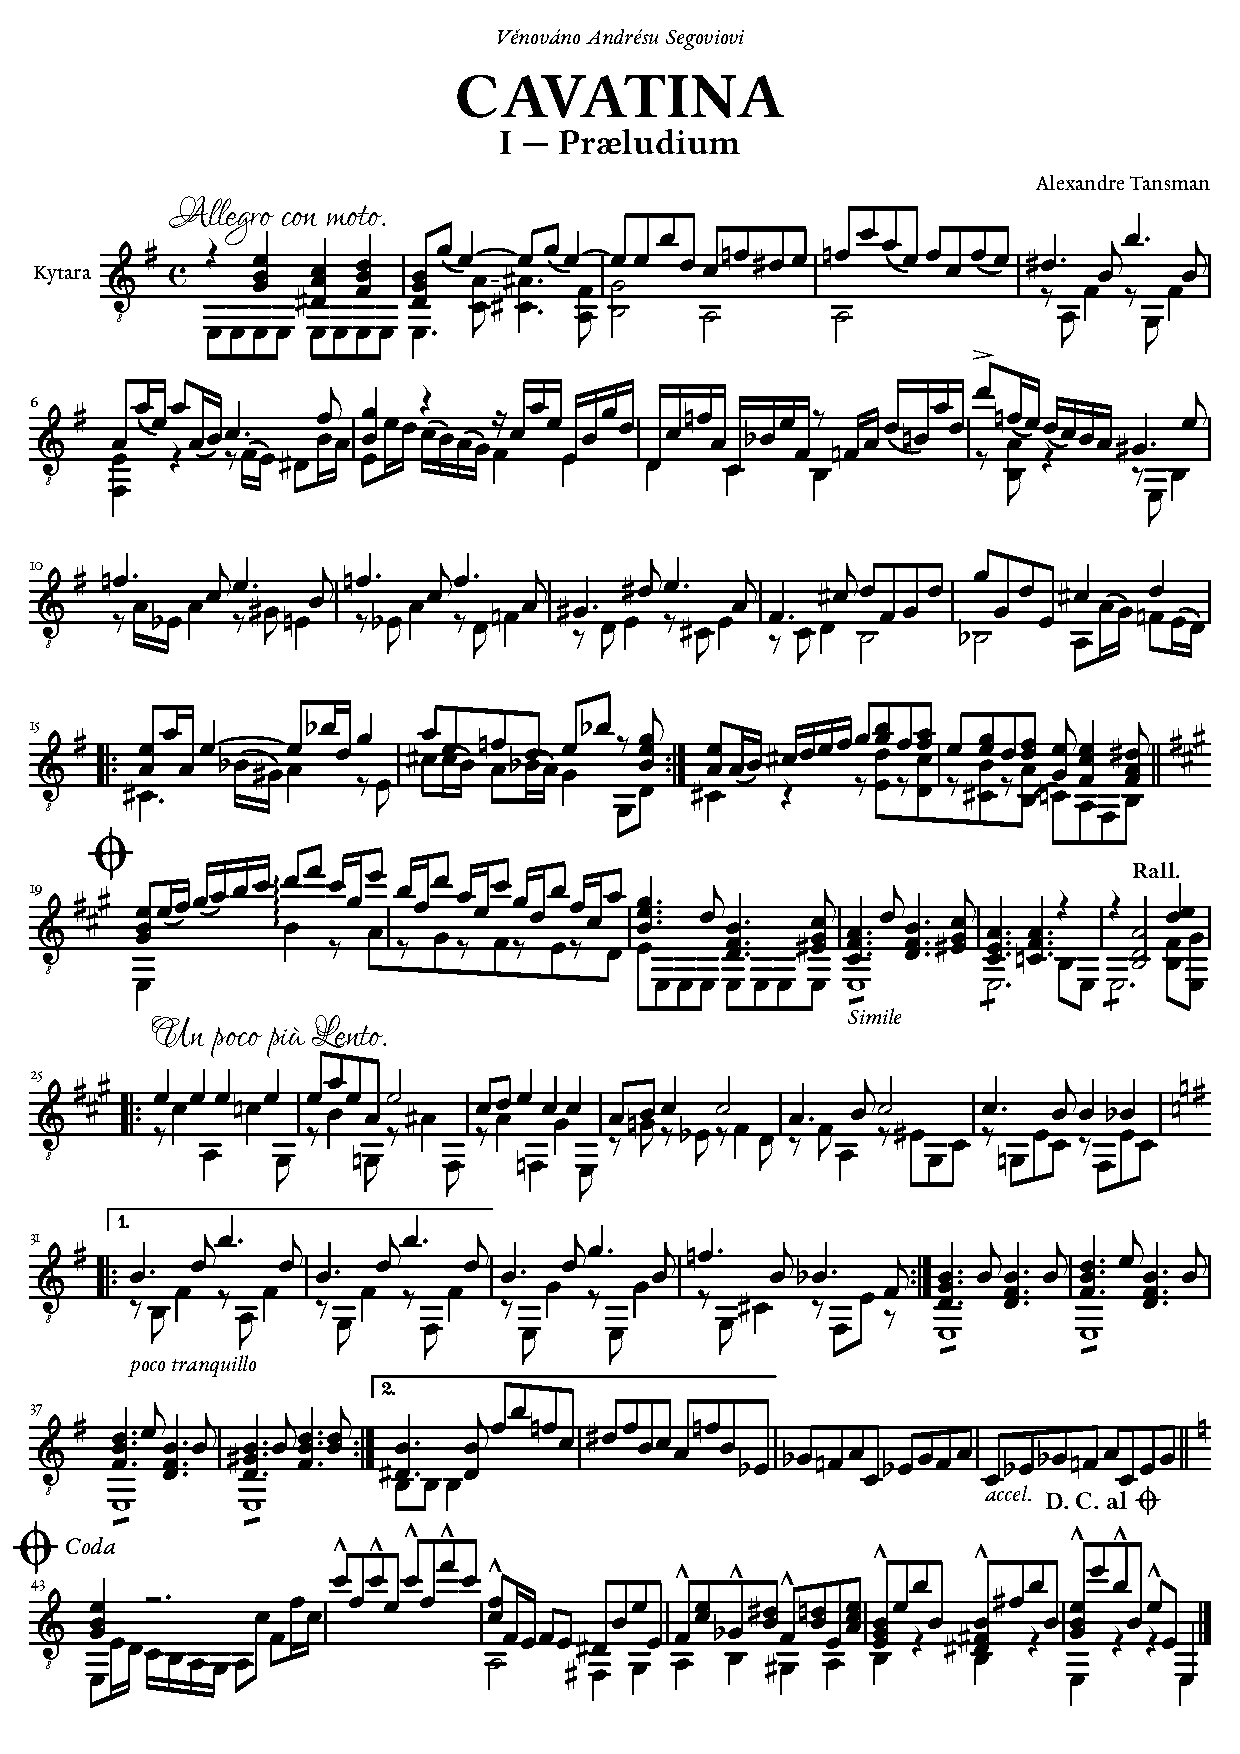
\includepdf{praeludium.pdf}

\includepdfmerge[nup=1x2]{sarabande.pdf,barcarole.pdf}

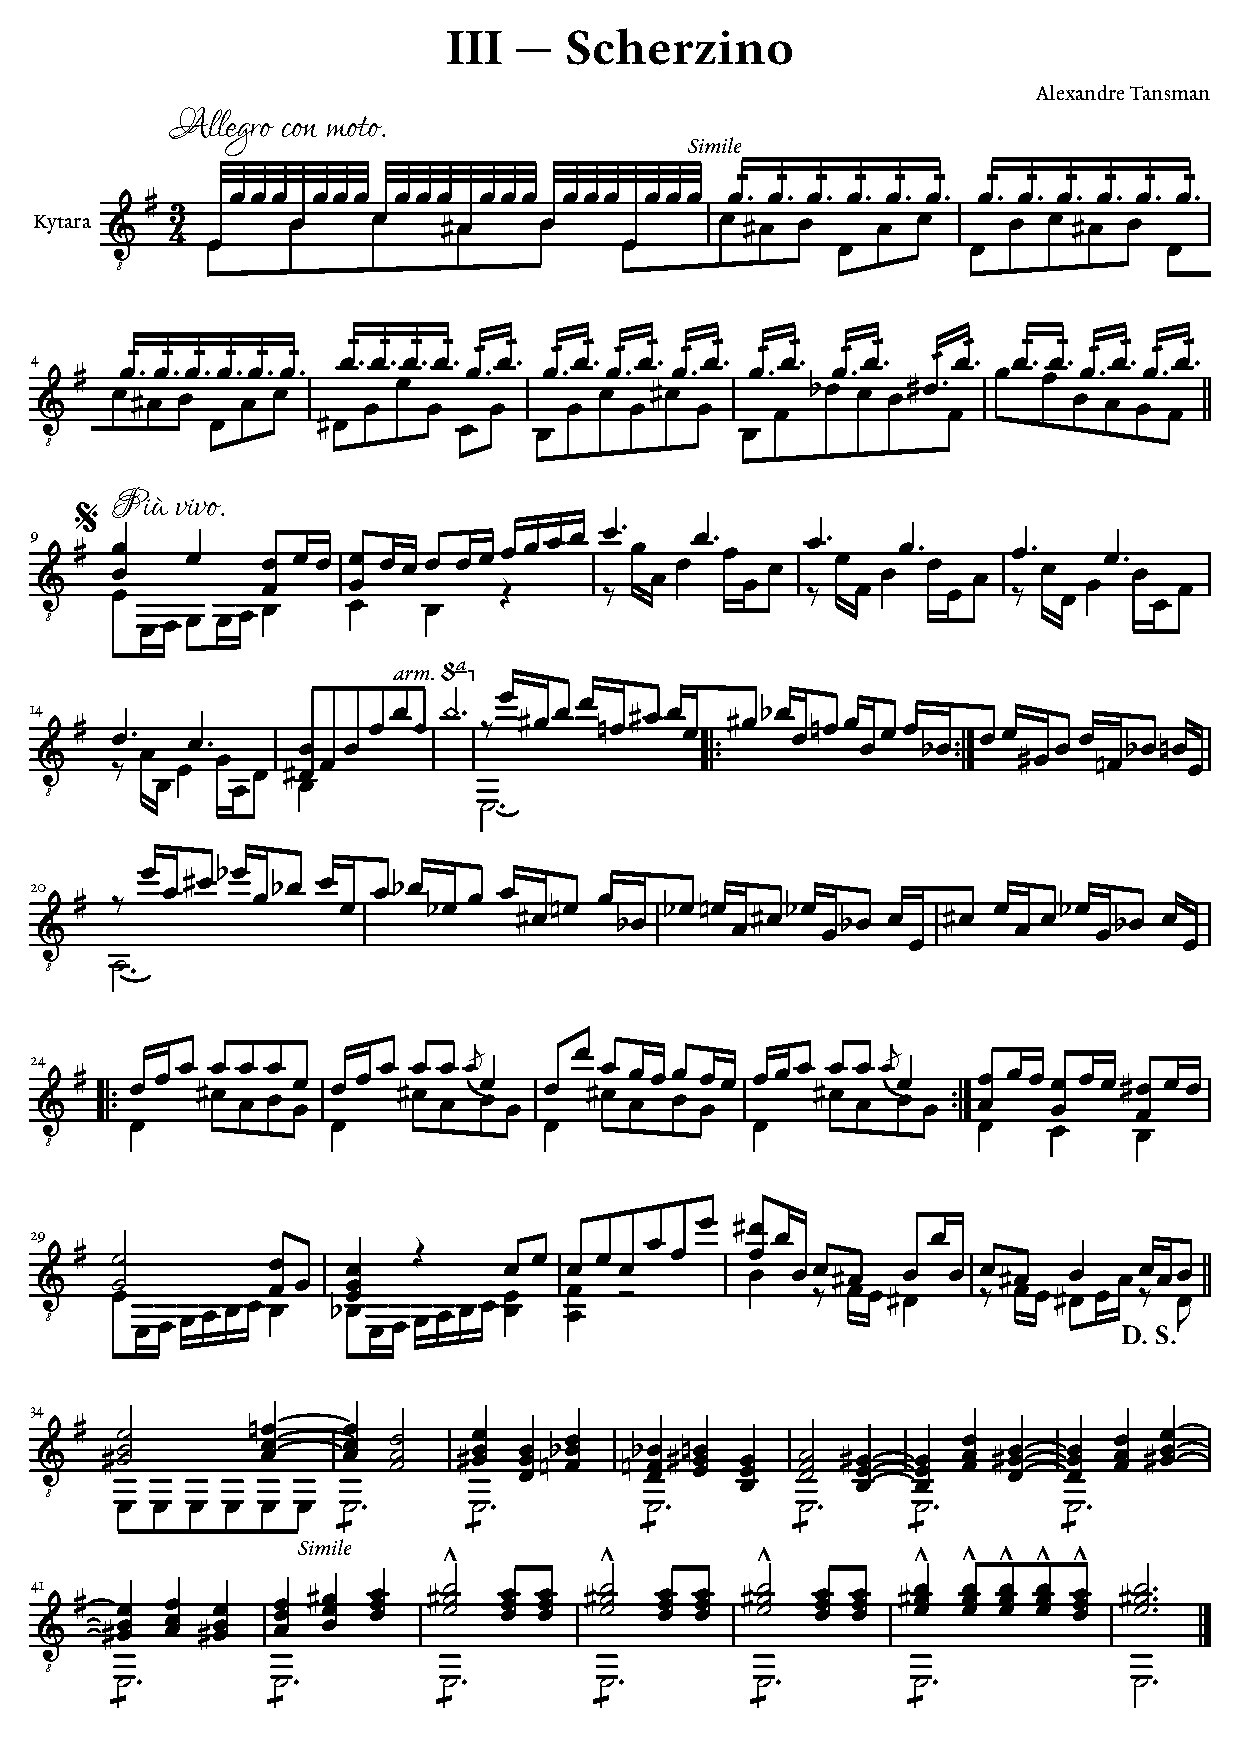
\includepdf{scherzino.pdf}

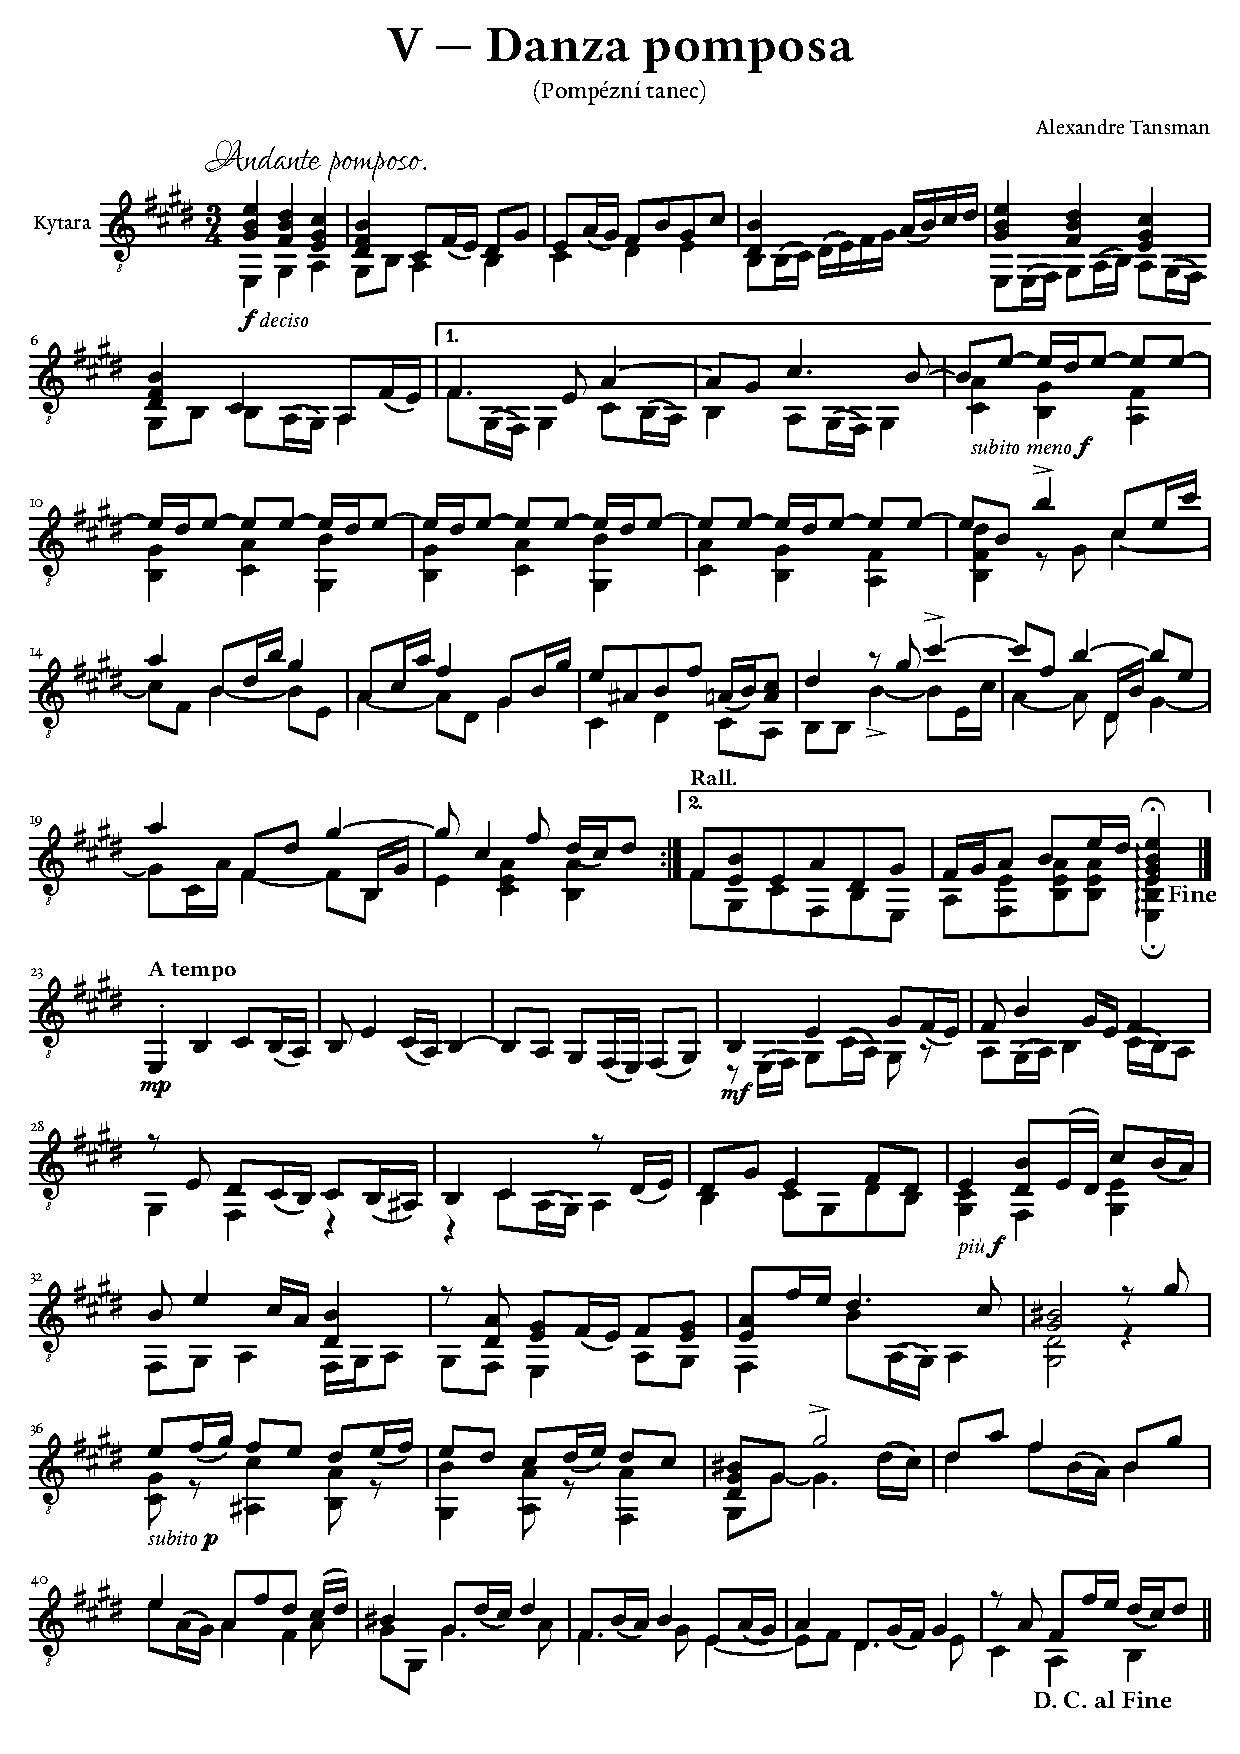
\includepdf{danza-pomposa.pdf}
\end{document}
